\documentclass[12pt,a4paper,parskip]{scrartcl}
\usepackage[utf8]{inputenc}
\usepackage[T1]{fontenc}
\usepackage[ngerman]{babel}
\usepackage{lmodern}
\usepackage[babel,german=guillemets]{csquotes}
\usepackage[backend=bibtex8]{biblatex}
\bibliography{baclit110414}
\usepackage{amsmath}
\usepackage{amsfonts}
\usepackage{amssymb}
\usepackage{mathabx}
\usepackage{makeidx}
\usepackage{graphicx}
\usepackage{url}
\usepackage[locale=DE]{siunitx}%SI Einheiten etc.
\usepackage[german]{fancyref}%möglicherweise rausnehmen oder justieren
\usepackage{booktabs} %Tabellen Horizontale Linier dick darstellen
\usepackage{rotating}
\usepackage{lscape}
\usepackage{subfig}
\usepackage{here}
\usepackage{color}
\usepackage[margin=10pt,font={small,sf,it},indention=.4cm,labelfont=bf,format=plain,width=.75\textwidth,labelfont={color=blue,bf}]{caption}

\usepackage{mdwlist}
\usepackage{morefloats}




\begin{document}
\maketitle
\begin{figure}[hbtp]
\centering
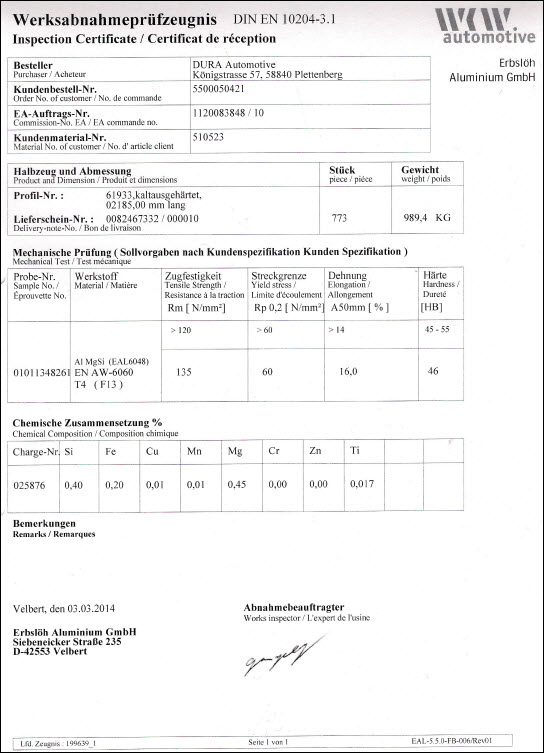
\includegraphics[width=.8\textwidth]{F13Datenblatt.jpg}
\caption{F13 Datenblatt}
\end{figure}
\begin{figure}[hbtp]
\centering
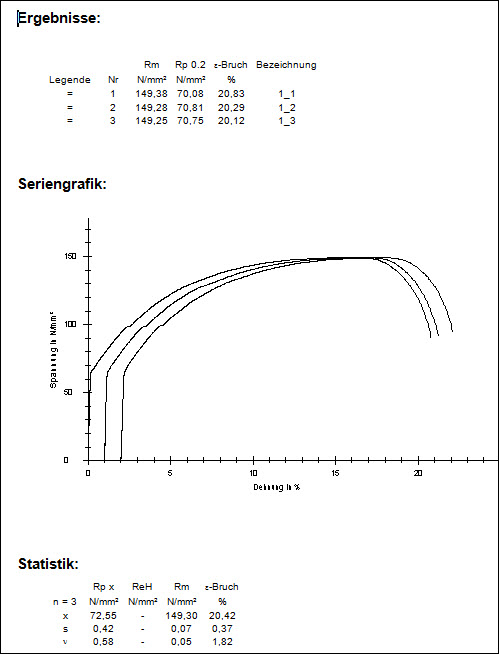
\includegraphics[width=1\textwidth]{F13Labor.jpg}
\caption{F13 Labor}
\end{figure}
\begin{figure}[hbtp]
\centering
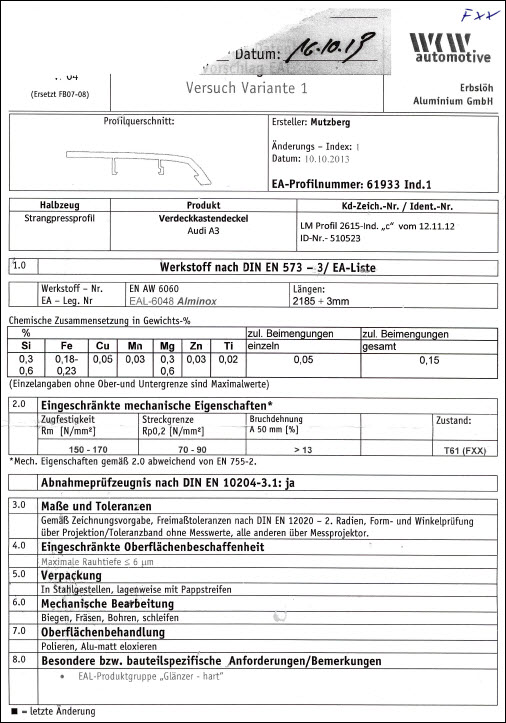
\includegraphics[width=1\textwidth]{FxxDatenblatt.jpg}
\caption{Fxx Datenblatt}
\end{figure}
\begin{figure}[hbtp]
\centering
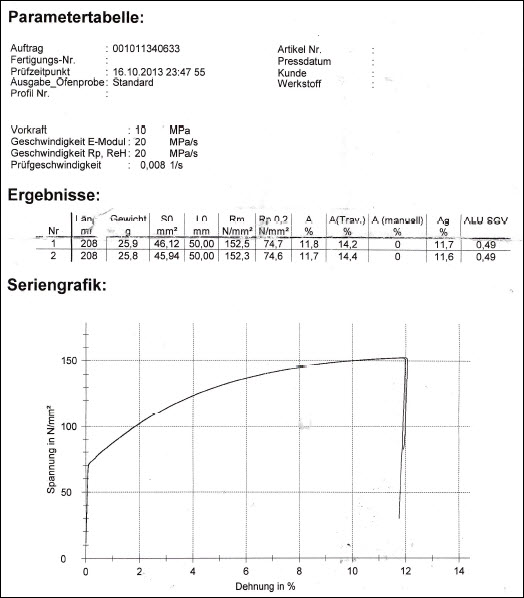
\includegraphics[width=1\textwidth]{FxxLabor.jpg}
\caption{Fxx Labor}
\end{figure}
\begin{figure}[hbtp]
\centering
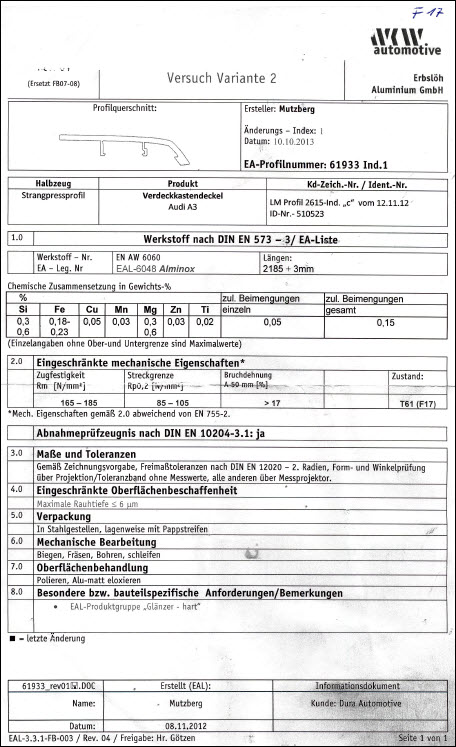
\includegraphics[width=1\textwidth]{F17Datenblatt.jpg}
\caption{F17 Datenblatt}
\end{figure}
\begin{figure}[hbtp]
\centering
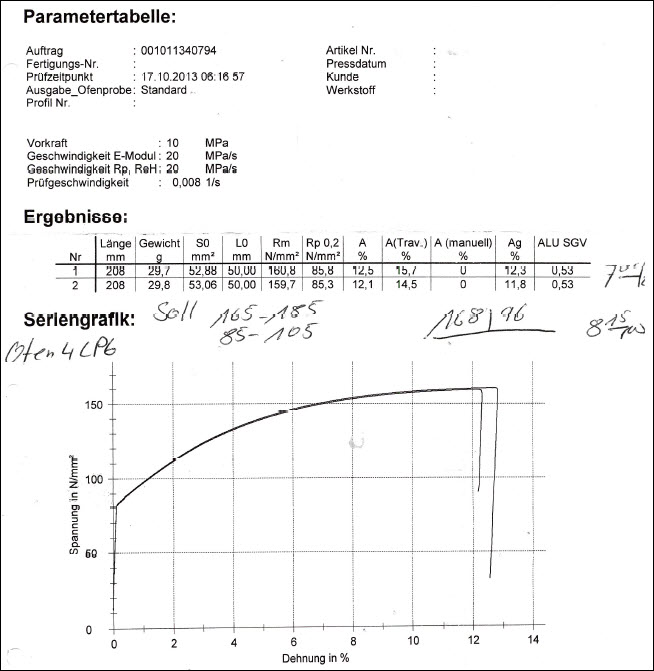
\includegraphics[width=1\textwidth]{F17Labor.jpg}
\caption{F17 Labor}
\end{figure}
\begin{figure}[hbtp]
\centering
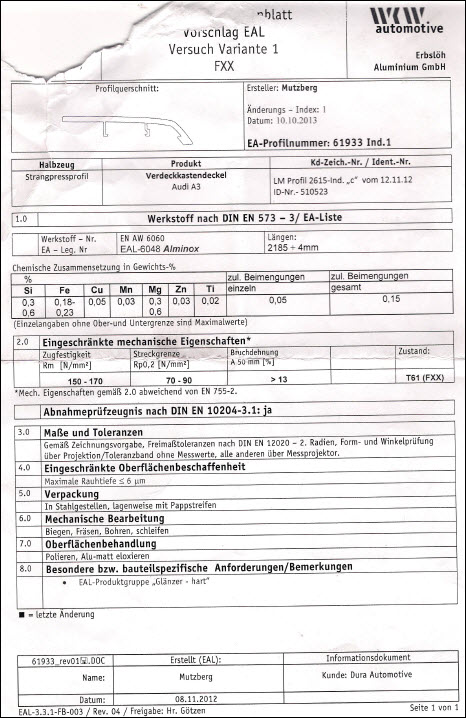
\includegraphics[width=1\textwidth]{nFxxDatenblatt.jpg}
\caption{nFxx Datenblatt}
\end{figure}
\begin{figure}[hbtp]
\centering
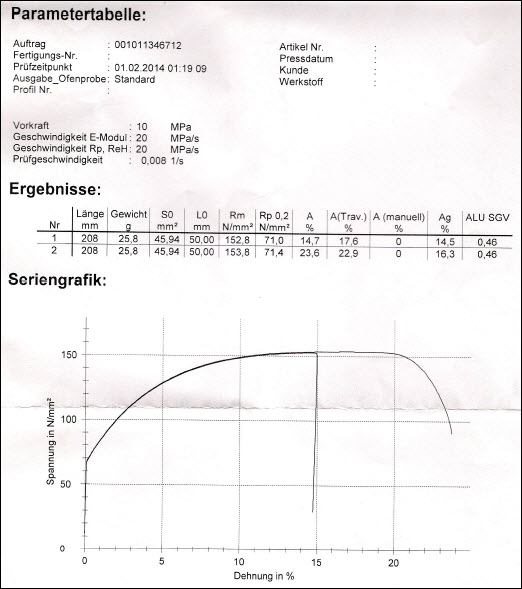
\includegraphics[width=1\textwidth]{nFxxLabor.jpg}
\caption{nFxx Labor}
\end{figure}
\begin{figure}[hbtp]
\centering
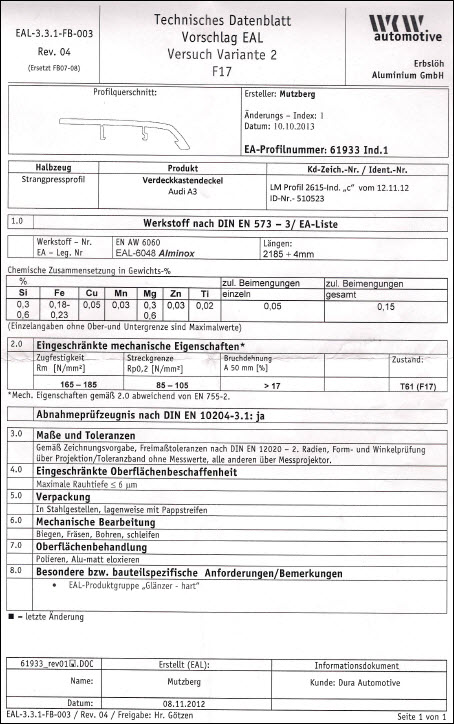
\includegraphics[width=1\textwidth]{nF17Datenblatt.jpg}
\caption{nF17 Datenblatt}
\end{figure}
\begin{figure}[hbtp]
\centering
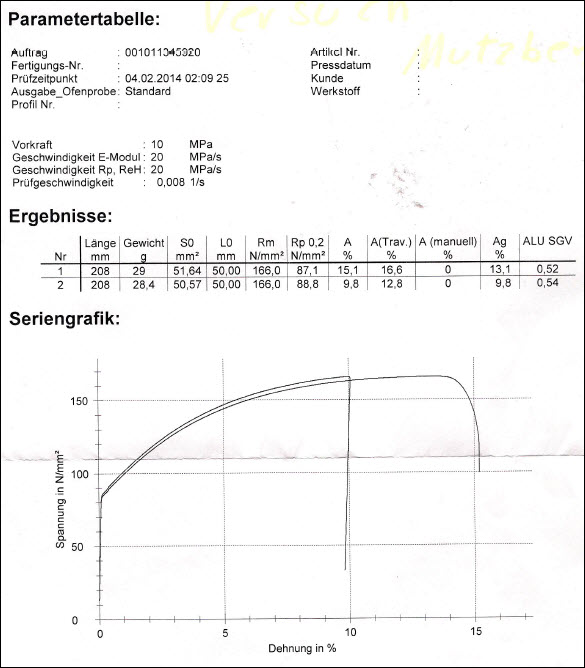
\includegraphics[width=1\textwidth]{nF17Labor.jpg}
\caption{nF17 Labor}
\end{figure}
\begin{figure}[hbtp]
\centering
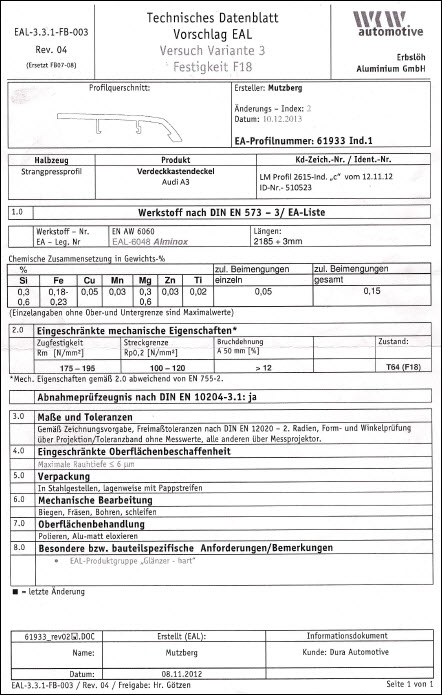
\includegraphics[width=1\textwidth]{F18Datenblatt.jpg}
\caption{F18 Datenblatt}
\end{figure}
\begin{figure}[hbtp]
\centering
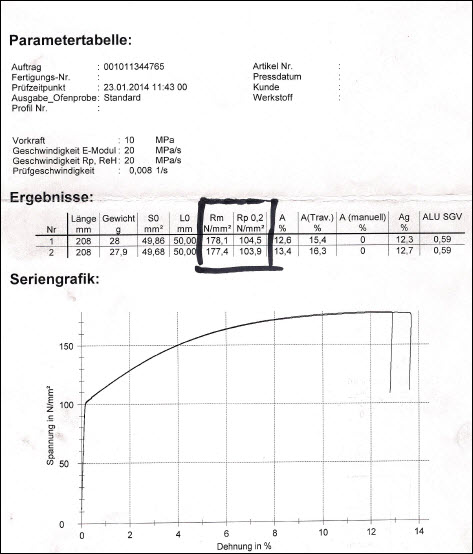
\includegraphics[width=1\textwidth]{F18Labor.jpg}
\caption{F18 Labor}
\end{figure}
\begin{figure}[hbtp]
\centering
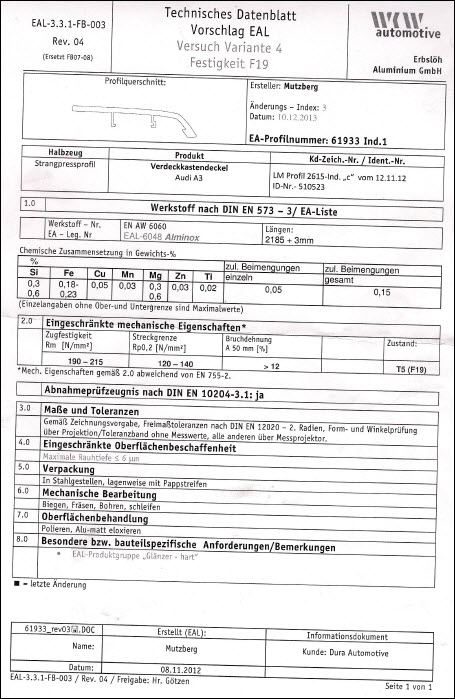
\includegraphics[width=1\textwidth]{F19Datenblatt.jpg}
\caption{F19 Datenblatt}
\end{figure}
\begin{figure}[hbtp]
\centering
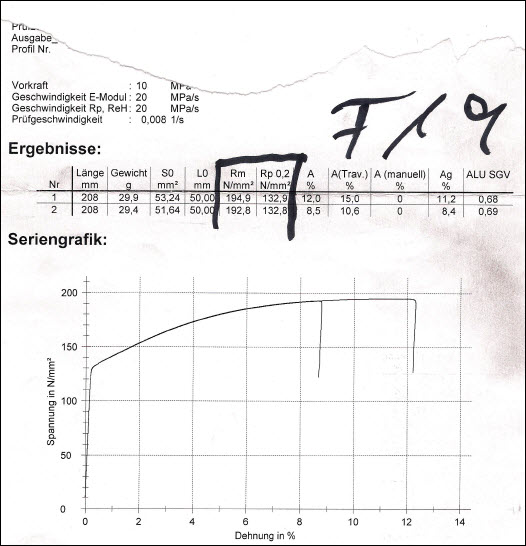
\includegraphics[width=1\textwidth]{F19Labor.jpg}
\caption{F19 Labor}
\end{figure}
\begin{figure}[hbtp]
\centering
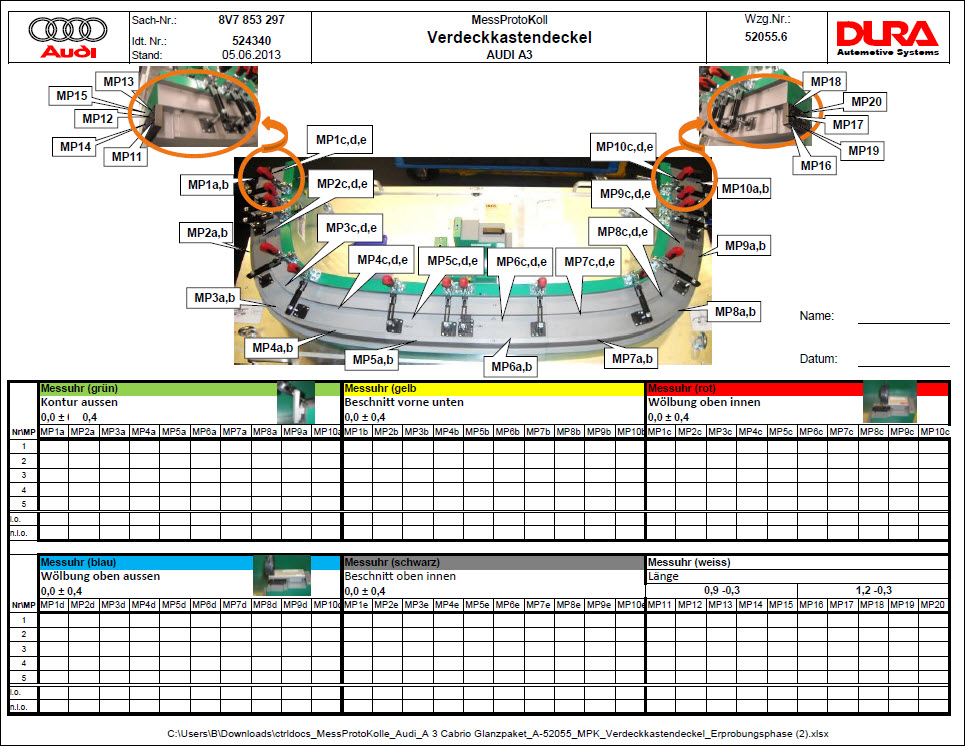
\includegraphics[width=1\textwidth]{MessblattOriginal.jpg}
\caption{Original Messblatt}
\end{figure}
\begin{figure}[hbtp]
\centering
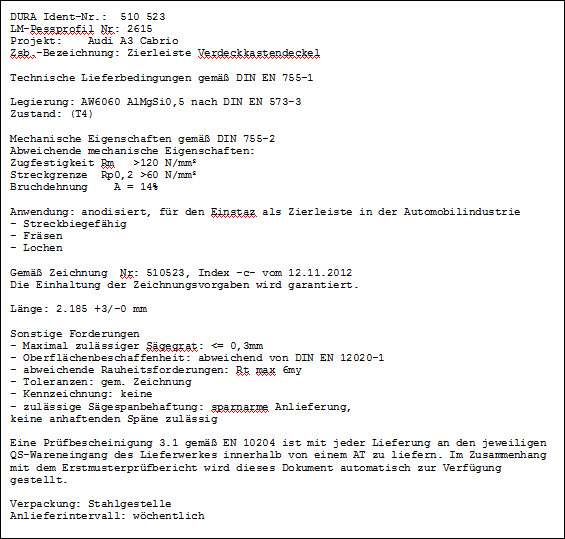
\includegraphics[width=1\textwidth]{Bestelltext.jpg}
\caption{Bestelltext}
\end{figure}
\begin{figure}[hbtp]
\centering
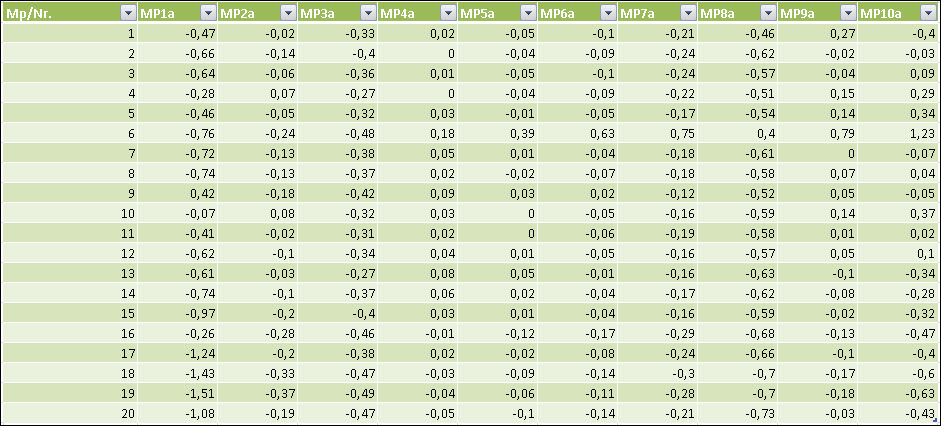
\includegraphics[width=1\textwidth]{F13Bieg.jpg}
\caption{Messwerte Streckbiegen "`Kontur aussen"' F13}
\end{figure}
\begin{figure}[hbtp]
\centering
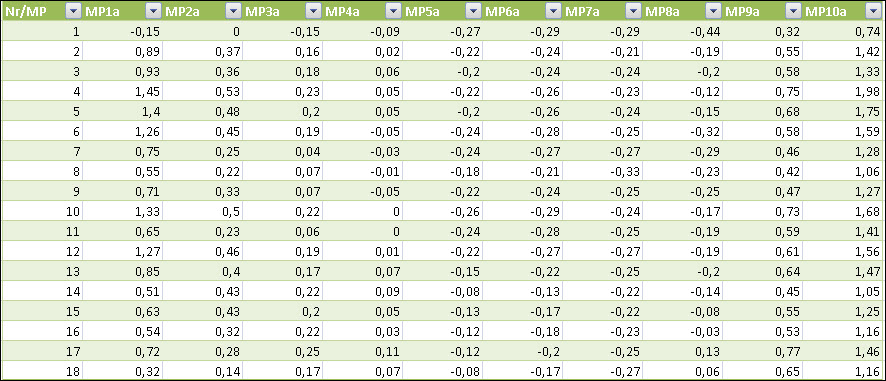
\includegraphics[width=1\textwidth]{FxxBieg.jpg}
\caption{Messwerte  Streckbiegen "`Kontur aussen"' Fxx}
\end{figure}
\begin{figure}[hbtp]
\centering
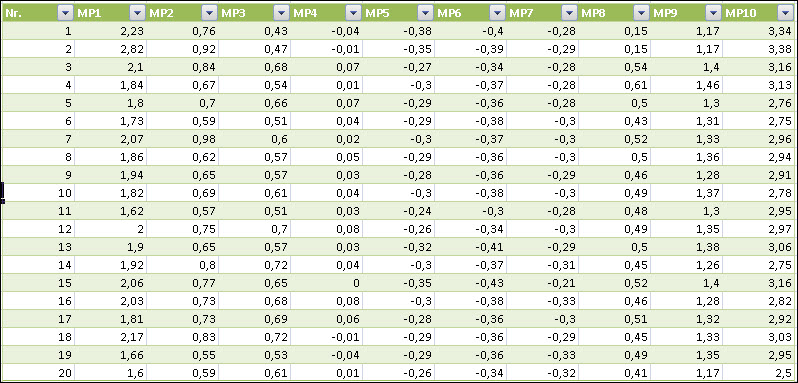
\includegraphics[width=1\textwidth]{F17Bieg.jpg}
\caption{Messwerte Streckbiegen "`Kontur aussen"' F17}
\end{figure}
\begin{figure}[hbtp]
\centering
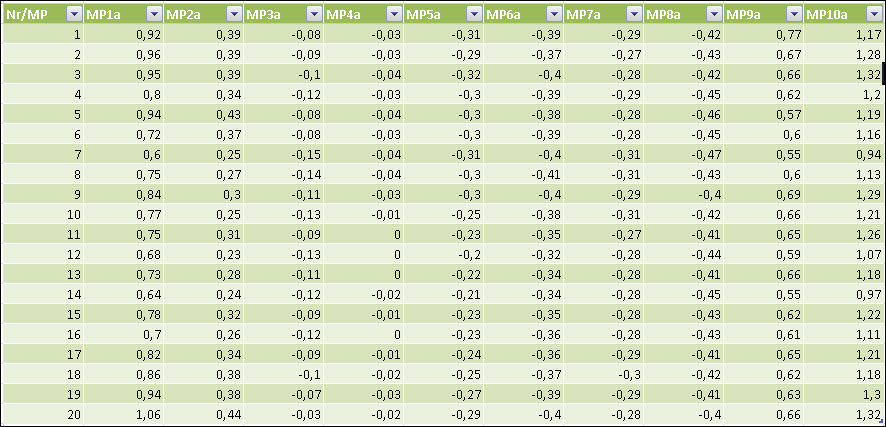
\includegraphics[width=1\textwidth]{nFxxBieg.jpg}
\caption{Messwerte Streckbiegen "`Kontur aussen"' nFxx}
\end{figure}
\begin{figure}[hbtp]
\centering
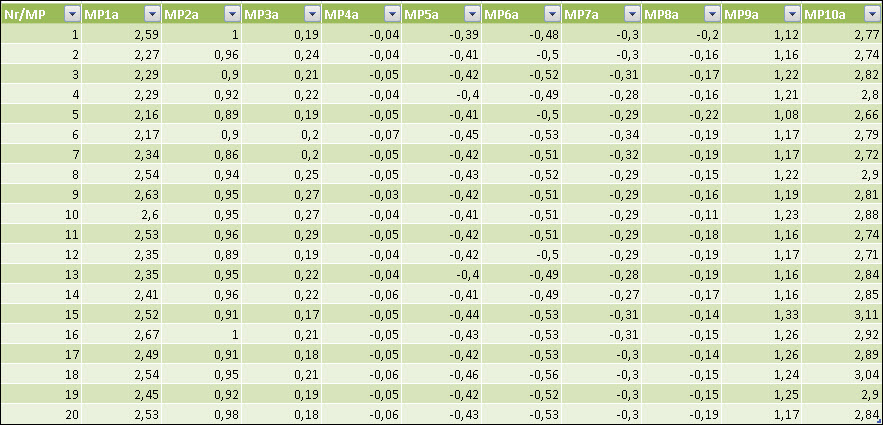
\includegraphics[width=1\textwidth]{nF17Bieg.jpg}
\caption{Messwerte Streckbiegen "`Kontur aussen"' nF17}
\end{figure}
\begin{figure}[hbtp]
\centering
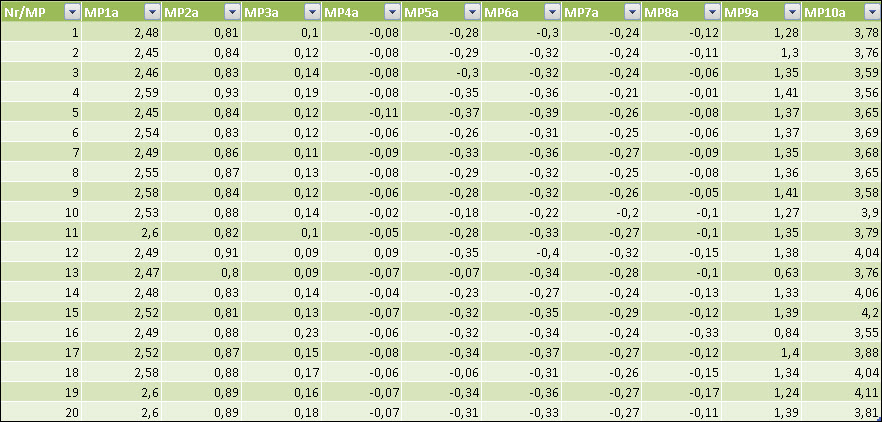
\includegraphics[width=1\textwidth]{F18Bieg.jpg}
\caption{Messwerte Streckbiegen "`Kontur aussen"' F18}
\end{figure}
\begin{figure}[hbtp]
\centering
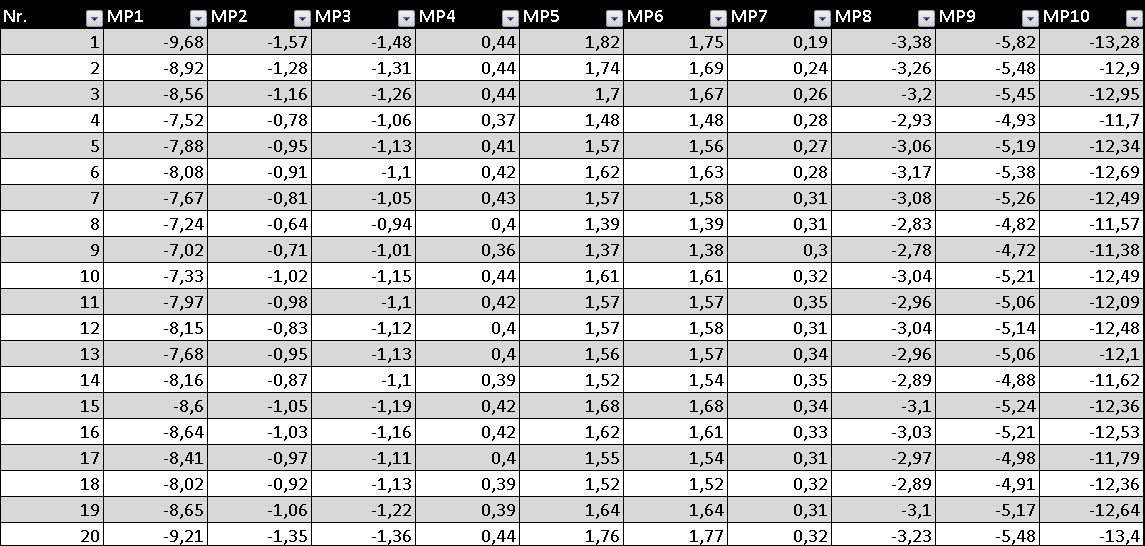
\includegraphics[width=1\textwidth]{F19Bieg.jpg}
\caption{Messwerte Streckbiegen "`Kontur aussen"' F19}
\end{figure}
\begin{figure}[hbtp]
\centering
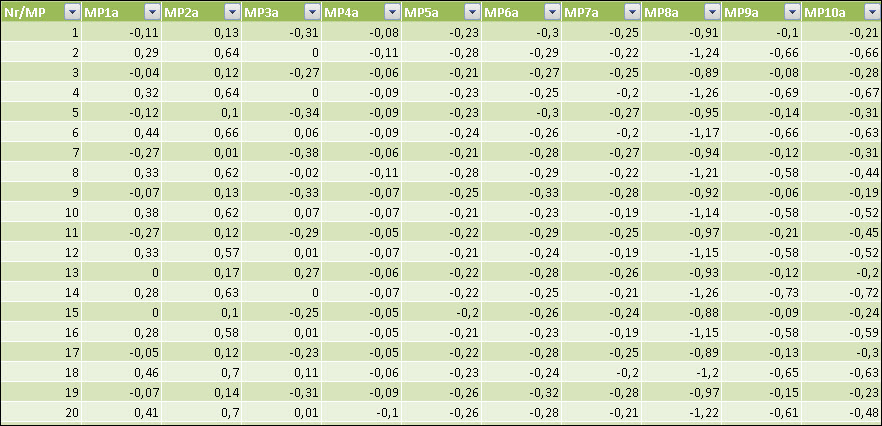
\includegraphics[width=1\textwidth]{F13fraes.jpg}
\caption{Messwerte Fräsen "`Kontur aussen"' F13 }
\end{figure}

\clearpage

\begin{figure}[hbtp]
\centering
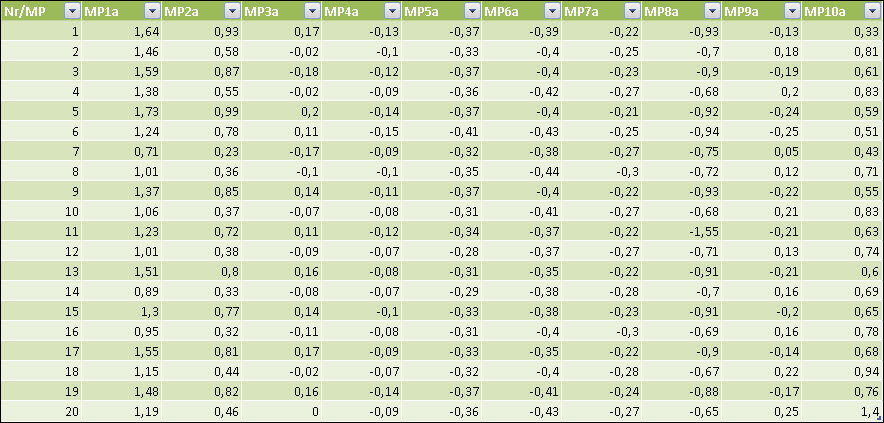
\includegraphics[width=1\textwidth]{Fxxfraes.jpg}
\caption{Messwerte Fräsen "`Kontur aussen"' Fxx}
\end{figure}
\begin{figure}[hbtp]
\centering
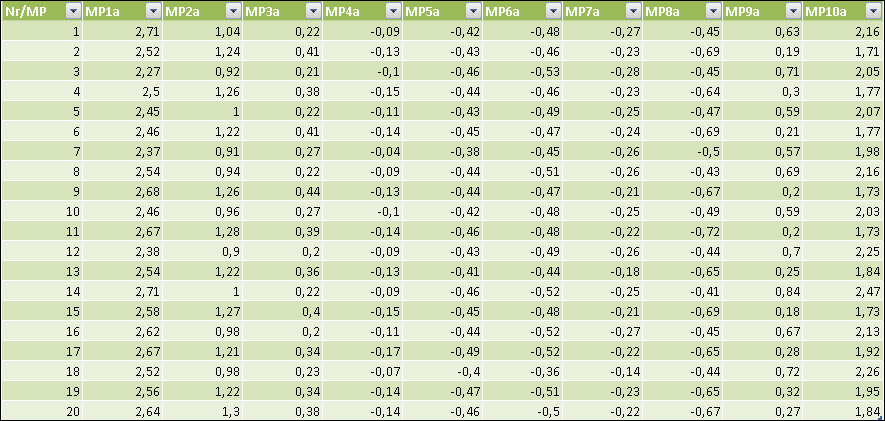
\includegraphics[width=1\textwidth]{F17fraes.jpg}
\caption{Messwerte Fräsen "`Kontur aussen"' F17}
\end{figure}
\begin{figure}[hbtp]
\centering
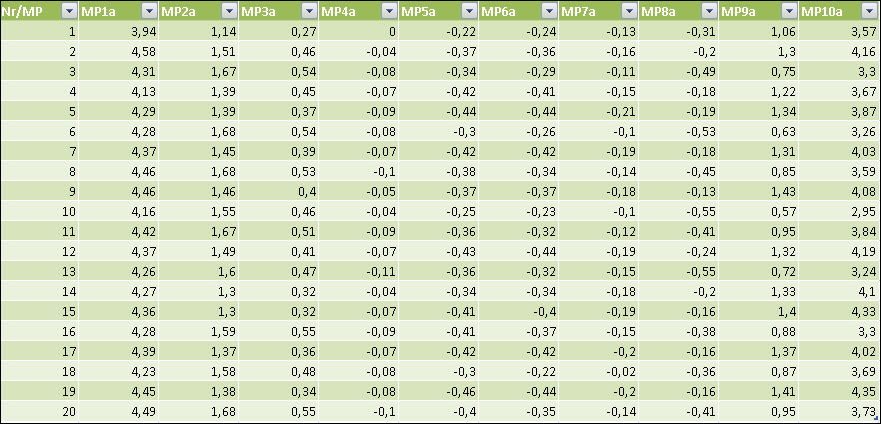
\includegraphics[width=1\textwidth]{F18fraes.jpg}
\caption{Messwerte Fräsen "`Kontur aussen"' F18}
\end{figure}
\begin{figure}[hbtp]
\centering
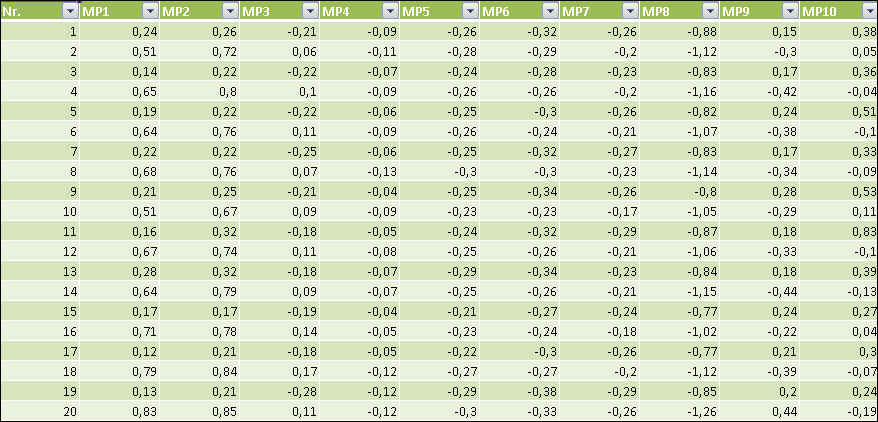
\includegraphics[width=1\textwidth]{F13polier.jpg}
\caption{Messwerte Polieren "`Kontur aussen"' F13}
\end{figure}
\begin{figure}[hbtp]
\centering
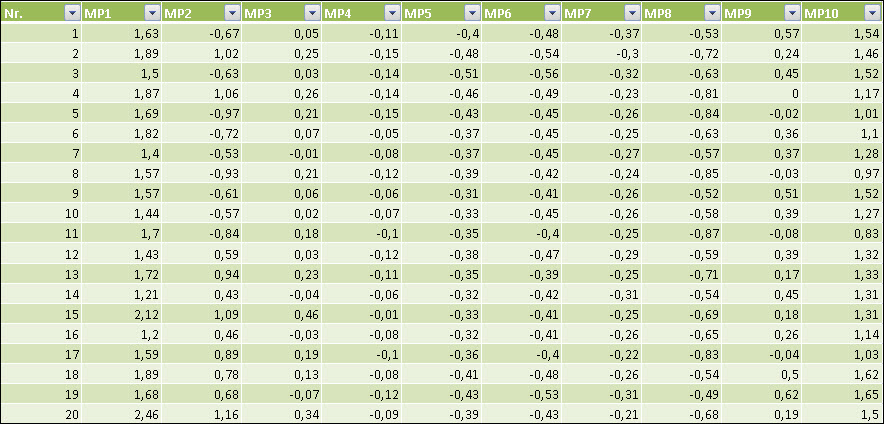
\includegraphics[width=1\textwidth]{Fxxpolier.jpg}
\caption{Messwerte Polieren "`Kontur aussen"' Fxx}
\end{figure}
\begin{figure}[hbtp]
\centering
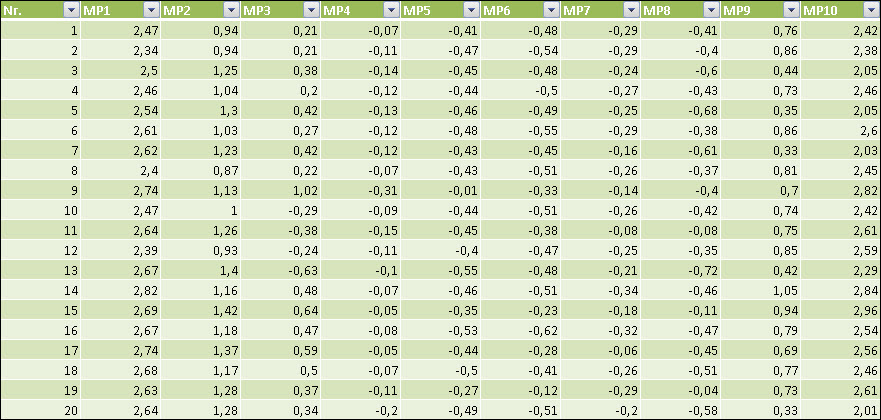
\includegraphics[width=1\textwidth]{F17polier.jpg}
\caption{Messwerte Polieren "`Kontur aussen"' F17}
\end{figure}
\begin{figure}[hbtp]
\centering
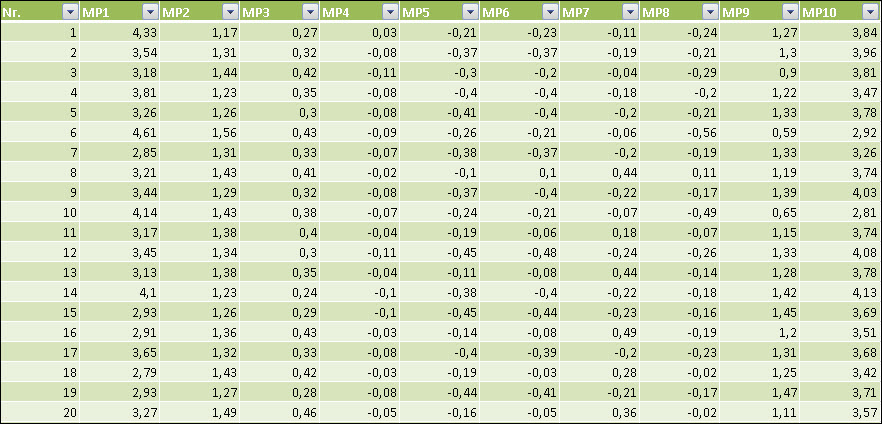
\includegraphics[width=1\textwidth]{F18polier.jpg}
\caption{Messwerte Polieren "`Kontur aussen"' F18}
\end{figure}
\begin{figure}[hbtp]
\centering
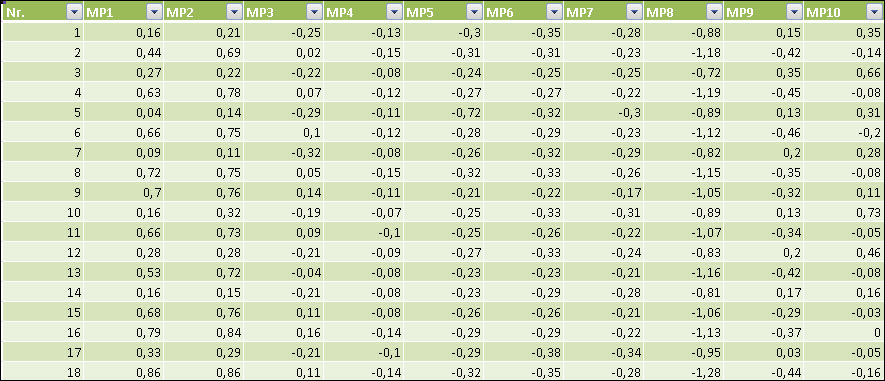
\includegraphics[width=1\textwidth]{F13elox.jpg}
\caption{Messwerte Eloxieren "`Kontur aussen"' F13}
\end{figure}
\begin{figure}[hbtp]
\centering
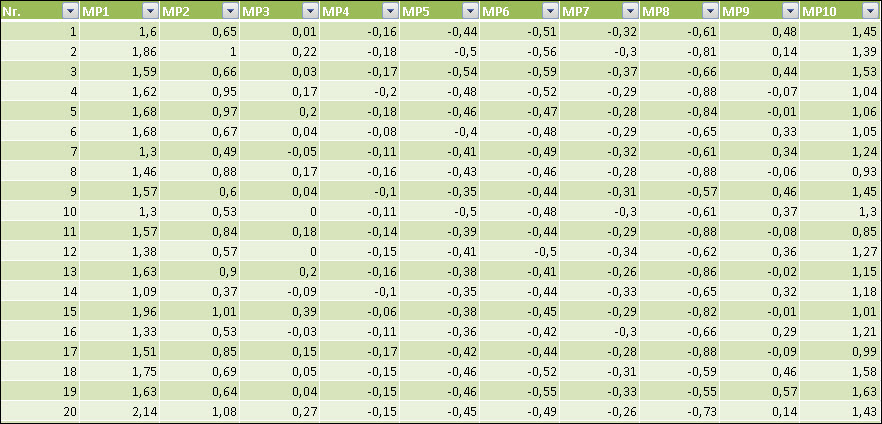
\includegraphics[width=1\textwidth]{Fxxelox.jpg}
\caption{Messwerte Eloxieren "`Kontur aussen"' Fxx}
\end{figure}
\begin{figure}[hbtp]
\centering
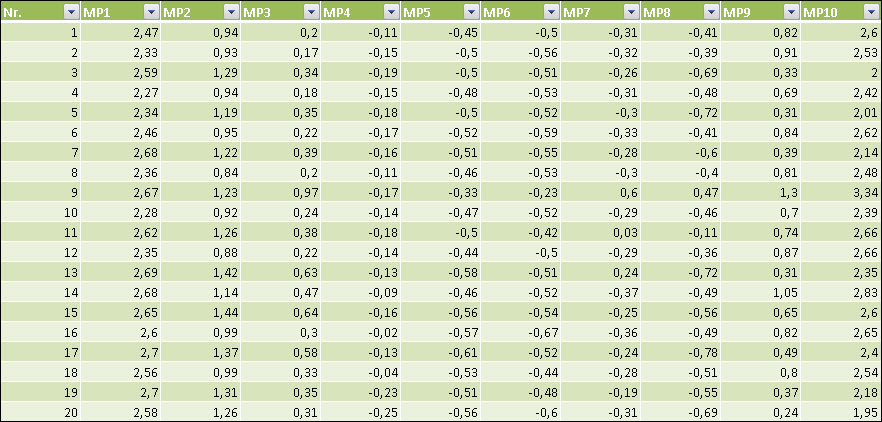
\includegraphics[width=1\textwidth]{F17elox.jpg}
\caption{Messwerte Eloxieren "`Kontur aussen"' F17}
\end{figure}
\begin{figure}[hbtp]
\centering
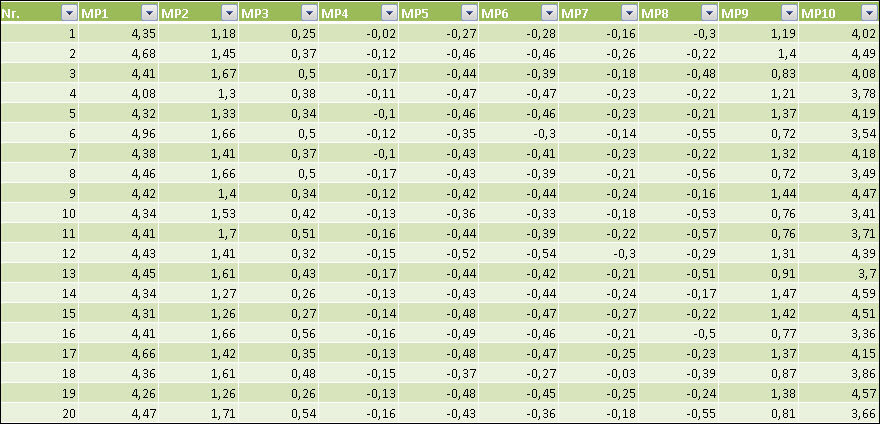
\includegraphics[width=1\textwidth]{F18elox.jpg}
\caption{Messwerte Eloxieren "`Kontur aussen"' F18}
\end{figure}
\begin{figure}[hbtp]
\centering
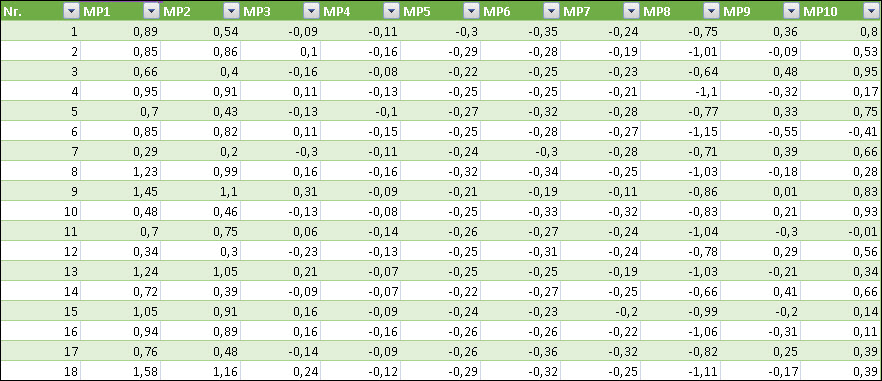
\includegraphics[width=1\textwidth]{F13durapro.jpg}
\caption{Messwerte DURApro "`Kontur aussen"' F13}
\end{figure}
\begin{figure}[hbtp]
\centering
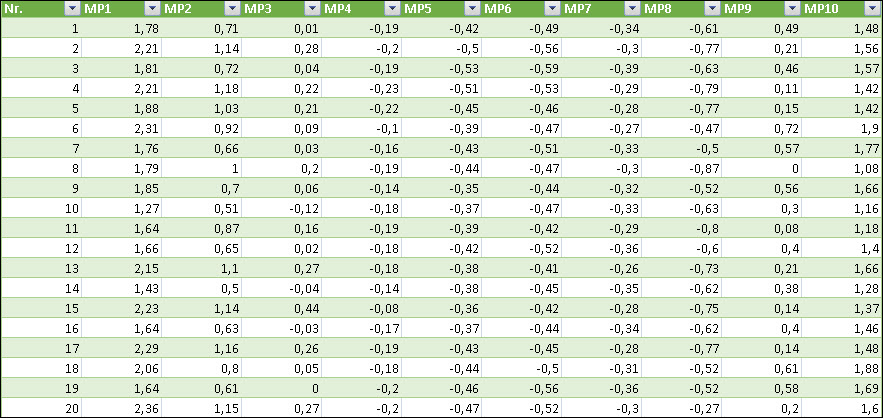
\includegraphics[width=1\textwidth]{Fxxdurapro.jpg}
\caption{Messwerte DURApro "`Kontur aussen"' Fxx}
\end{figure}
\begin{figure}[hbtp]
\centering
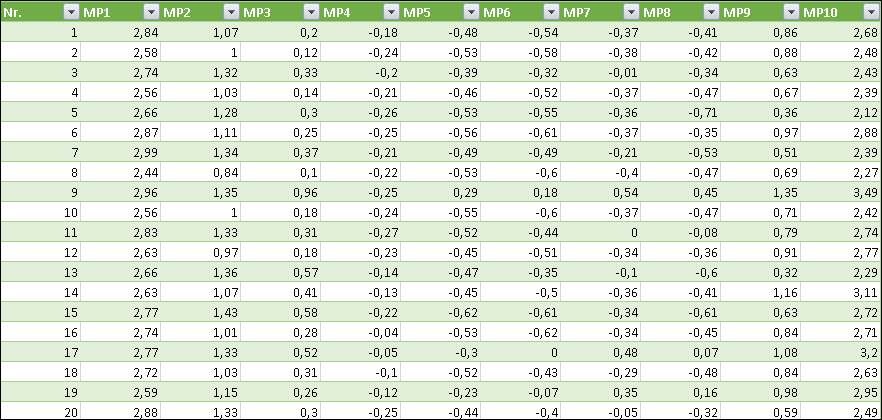
\includegraphics[width=1\textwidth]{F17durapro.jpg}
\caption{Messwerte DURApro "`Kontur aussen"' F17}
\end{figure}
\begin{figure}[hbtp]
\centering
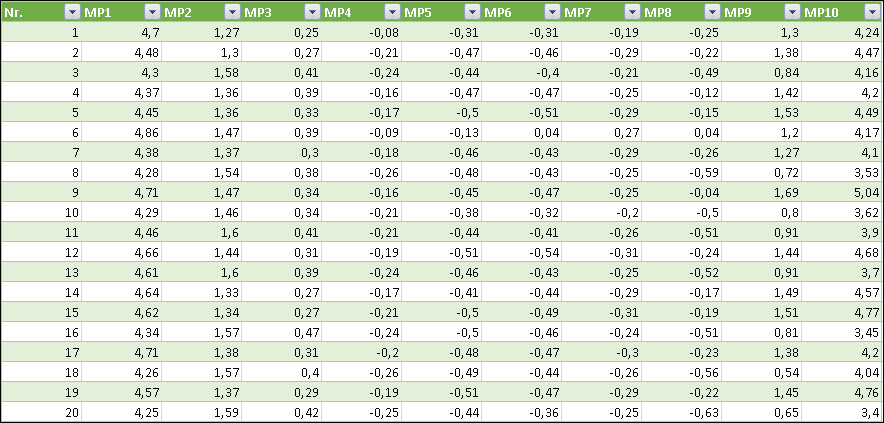
\includegraphics[width=1\textwidth]{F18durapro.jpg}
\caption{Messwerte DURApro "`Kontur aussen"' F18}
\end{figure}













































   


\end{document}  
